% This file is iccc.tex.  It contains the formatting instructions for and acts as a template for submissions to ICCC.  It borrows liberally from the AAAI and IJCAI formats and instructions.  It uses the files iccc.sty, iccc.bst and iccc.bib, the first two of which also borrow liberally from the same sources. The format has been updated for the ICCC2022 to include a new, mandatory section to be included in camera-ready manuscripts.


\documentclass[letterpaper]{article}
\usepackage{iccc}


\usepackage{times}
\usepackage{helvet}
\usepackage{courier}
\usepackage{amsmath}
\usepackage{musicography}
\usepackage{graphicx}
\usepackage[font=small,skip=0pt]{caption}

\pdfinfo{
/Title (Formatting Instructions for Authors)
/Subject (Proceedings of ICCC)
/Author (ICCC)}
% The file iccc.sty is the style file for ICCC proceedings.
%
\title{Converting DNA to Music: Sonifying Splicing and Translation}
\author{Ilana Shapiro\\
Computer Science Department\\
Pomona College\\
Claremont, CA 91711 USA\\
issa2018@mymail.pomona.edu\\
}
\setcounter{secnumdepth}{0}

\begin{document} 
\maketitle
\begin{abstract}
The sonification of genetic material is a little-explored mode of unconventional computation that bridges the divide between bioinformatics, computer science, and music, allowing bioinformaticians to perceptualize their data in a novel and illuminating manner. This paper presents BioMus, an original model for converting DNA to musical data in the form of MIDI piano chords. Gene sequences are sourced from Ensembl, a genome database of the European Bioinformatics Institute, and are parsed into exons and and introns. Exons are further parsed into their 5' and 3' untranslated regions (UTRs) and their CDS (CoDing Sequence, i.e. the spliced exons constituting the amino acid-coding sequence after UTRs are removed). Then, each codon in a CDS region is mapped to a major chord, individual nucleotides in introns are mapped to diminished chords, and individual nucleotides in UTRs are mapped to minor chords. CDS codons are mapped to chords based on the amino acids they code for, and rhythmic alterations indicate when CDS codons are broken across splice sites. To further emphasize protein-coding regions, all CDS chords are also at a higher volume. By mapping nucleotides and codons to chords and analyzing genetic material as music, BioMus thus gives scientists a novel means to conceptualize the process of biological splicing and translation.

ONE PARAGRAPH, max 250words
\end{abstract}

\section{Introduction}

\section{Related Work}

Ingalls et al. present 

\section{Converting DNA to Music}
\subsection{Obtaining Genetic Data}
BioMus's process of DNA sonification begins with the user specifying a desired species and gene. This information is passed to Ensembl's REST API to obtain Ensembl's choromomal coordinates of the gene's exons. These coordinates are sourced from the gene's \textit{canonical transcript}, the gene's transcript in Ensembl that is overall the most conserved and highly expressed, has the longest CDS, and is also represented in other major databases such as the NCBI \cite{ensembl_transcript_flags}. The exon coordinates also define the chromosomal coordinates of the intervening introns. Each pair of exon and intron coordinates is passed back to the Ensembl REST API to obtain the nucleotide sequences for each region, and the result is a list of sequence regions alternating exons and introns. For instance, consider the abbreviated sequence obtained from Ensembl for the \textit{Homo sapiens} (human) TP53 tumor suppressor gene in Figure \ref{fig:pre_processed_seq_homo_sapiens_tp53}. Ellipses indicate omitted nucleotides for the sake of example.

\begin{figure}[h!]
\centering
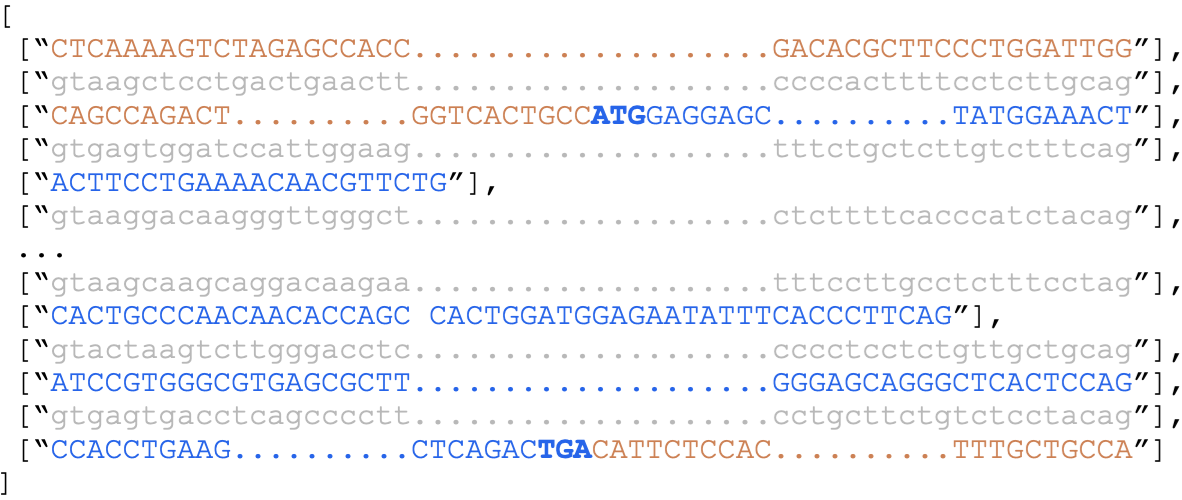
\includegraphics[width=0.48\textwidth]{images/pre_processed_seq_homo_sapiens_tp53_ABBREV}
  \caption{Homo sapiens}\label{fig:pre_processed_seq_homo_sapiens_tp53}
  \vspace{-3mm}
\end{figure}

Exons are in color, while introns are in grey. Within the exons, the orange regions are the UTRs, and the blue regions are the CDS. Notice how the CDS begins with the bolded start codon ATG and ends with the bolded stop codon TGA. 

Now, the goal is to extract the 5' UTR from the list. In order to ensure the correct CDS, is necessary to verify the 5' UTR with Ensemble, since it may include multiple ATG start codons that do not signal the start of the CDS. This is not necessary for the 3' UTR, since once we know we are in the CDS, the first stop codon will always signal the end of the CDS and the beginning of the 3' UTR. We obtain the 5' UTR from Ensembl by querying the Ensembl REST API for the cDNA (complementary DNA) sequence of the canonical transcript. cDNA is identical to the CDS, but includes the UTRs \cite{ensembl_glossary}. By requesting Ensembl to ``mask" the UTRs of the cDNA sequence by representing them in lowercase, we can successfully isolate the 5' UTR and extract it from the list in Figure \ref{fig:pre_processed_seq_homo_sapiens_tp53}. As seen in Figure \ref{fig:post_processed_seq_homo_sapiens_tp53}, we end up with a list of the 5' UTR regions (top), and a list of the CDS regions and introns (bottom).\cite{10.1162/artl_a_00325}

\begin{figure}[h!]
\centering
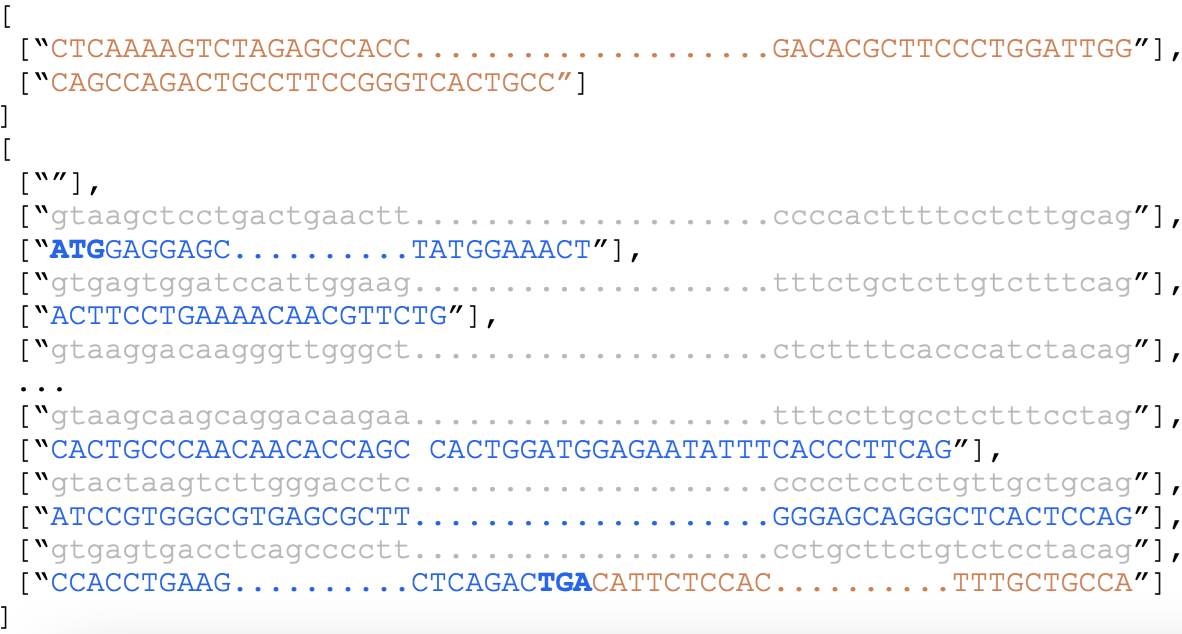
\includegraphics[width=0.48\textwidth]{images/post_processed_seq_homo_sapiens_tp53_ABBREV}
\vspace{-3mm}
  \caption{Homo sapiens}\label{fig:post_processed_seq_homo_sapiens_tp53}
  \vspace{-3mm}
\end{figure}

We now have all the tools necessary to translate the genetic data into music.

\subsection{Conversion to MIDI}

Next, a MIDI track is created using the MIDIUtil library with the tempo set to \musQuarter\;= 200 BPM, and the DNA sequence is transcribed to RNA with Biopython. Recall the bases used in RNA are adenine (A), cytosine (C), guanine (G) and uracil (U), and have the pairings C-G and A-U. BioMus defines the following mapping of individual bases to musical notes relative to the local key in Table  \ref{table:nucleotides}.

\begin{table}[h!]
\centering
\begin{tabular}{|l|l|}
\hline
C   & Tonic    \\ \hline
G,A & Mediant  \\ \hline
U   & Dominant \\ \hline
\end{tabular}
\caption{RNA Base Mappings}
\label{table:nucleotides}
\end{table}

The musical key is minor in non-coding regions and major in protein-coding regions, with the initial key set to C minor. Before the start codon AUG is encountered, individual nucleotides outline the 3 notes of minor triad of the local key (base pairs form dyads, or 2-note chords). Then, during translation, the key is major and the volume doubles. The
        key is determined by the codon (see the AMINOACIDS dictionary above). Individual nucleotides no longer determine the notes; this is now dictated
        by the codons. Each time the key changes based on the codon, the major triad of that key is played, until a stop codon is reached. Then we remain in
        the same minor key as the previous stop codon, but the volume is halved again and individual nucleotides once again outline the notes of the new
        minor triad. Then this process can repeat if another start codon is then encountered'


The tonic, mediant, and dom

Throughout this paper, the chosen gene for MIDI generation and analysis is TP53, which codes for the tumor suppressor protein p53. 

\begin{table}[h!]
\centering
\begin{tabular}{|l|l|l|}
\hline
AUG & \begin{tabular}[c]{@{}l@{}}Methionine/\\Start Codon\end{tabular} & C                         \\ \hline
AUU, AUC, AUA & Isoleucine                        & C\musSharp \\ \hline
AAA, AAG &  Lysine                      & D                         \\ \hline
ACU, ACC, ACA, ACG & Threonine                       & E\musFlat  \\ \hline
UUU, UUC & Phenylalanine                       & E                         \\ \hline
UGG & Tryptophan             & F                         \\ \hline
\begin{tabular}[c]{@{}l@{}}UUA, UUG, CUU, CUC, \\CUA, CUG\end{tabular}  & Leucine                       & F\musSharp \\ \hline
CAU, CAC & Histidine                       & G                         \\ \hline
GUU, GUC, GUA, GUG &  Valine                      & A\musFlat  \\ \hline
\end{tabular}
\caption{Essential Amino Acids}
\label{table:essential}
\end{table}

\begin{table}[h!]
\centering
\begin{tabular}{|l|l|l|}
\hline
AAU, AAC & Asparagine & A                        \\ \hline
GAU, GAC & Aspartate  & B\musFlat \\ \hline
GCU, GCC, GCA, GCG & Alanine    & B                        \\ \hline
\end{tabular}
\caption{Nonessential Amino Acids}
\label{table:nonessential}
\end{table}

\begin{table}[h!]
\centering
\begin{tabular}{|l|l|l|}
\hline
UAU, UAC & Tyrosine                & C \\ \hline
UGU, UGC & Cysteine                & D \\ \hline
\begin{tabular}[c]{@{}l@{}}UCC, UCU, UCA, UCG, \\ AGU,  AGC\end{tabular}  & Serine                  & E \\ \hline
\begin{tabular}[c]{@{}l@{}}AGA, AGG, CGU, CGC, \\ CGA, CGG\end{tabular}  & Arginine                & F \\ \hline
CCU,  CCC, CCA, CCG & Proline                 & G \\ \hline
CAA, CAG, GAA, GAG  & \begin{tabular}[c]{@{}l@{}}Glutamine/\\Glutamic acid\end{tabular}  & A \\ \hline
GGU, GGC, GGA, GGG & Glycine                 & B \\ \hline
\end{tabular}
\caption{Conditionally Essential Amino Acids}
\label{table:conditionally_essential}
\end{table}

\begin{table}[h!]
\centering
\begin{tabular}{|l|l|}
\hline
UAA & C \\ \hline
UAG & E \\ \hline
UGA & G \\ \hline
\end{tabular}
\caption{Stop Codons}
\label{table:stop_codons}
\end{table}

\section{Sample Music}

\section{Conclusion}
BioMus serves as a bridge between bioinformatics, computer science, and music by giving scientists the creative means to 


\section{Acknowledgments}

I am very grateful to Professor Zachary Dodds of Harvey Mudd College for his invaluable mentorship throughout this project.


\bibliographystyle{iccc}
\bibliography{iccc}


\end{document}
